\input{../YKY-preamble.tex}
\setmainfont[BoldFont=Alibaba_Sans_Regular.otf,ItalicFont=Alibaba_Sans_Light_Italic.otf]{Alibaba_Sans_Light.otf}

\usepackage[backend=biber]{biblatex}
\bibliography{../AGI-book}

\usepackage[active,tightpage]{preview}		% for continuous page(s)
\renewcommand{\PreviewBorder}{0.5cm}
\renewcommand{\thempfootnote}{\arabic{mpfootnote}}

\usepackage[absolute,overlay]{textpos}		% for page number on upper left corner

\usepackage{color}
\usepackage{mathtools}
\usepackage[hyperfootnotes=false]{hyperref}

% \usepackage[backend=biber,style=numeric]{biblatex}
% \bibliography{../AGI-book}
% \renewcommand*{\bibfont}{\footnotesize}

\usetikzlibrary{shapes}
\usepackage[export]{adjustbox}				% ??
\usepackage{verbatim} % for comments
% \usepackage{newtxtext,newtxmath}	% Times New Roman font

% \titleformat{\subsection}[hang]{\bfseries\large\color{blue}}{}{0pt}{} 
% \numberwithin{equation}{subsection}

\newcommand{\underdash}[1]{%
	\tikz[baseline=(toUnderline.base)]{
		\node[inner sep=1pt,outer sep=10pt] (toUnderline) {#1};
		\draw[dashed] ([yshift=-0pt]toUnderline.south west) -- ([yshift=-0pt]toUnderline.south east);
	}%
}%

\newcommand\reduline{\bgroup\markoverwith{\textcolor{red}{\rule[-0.5ex]{2pt}{0.4pt}}}\ULon}

%\DeclareSymbolFont{symbolsC}{U}{txsyc}{m}{n}
%\DeclareMathSymbol{\strictif}{\mathrel}{symbolsC}{74}
\DeclareSymbolFont{AMSb}{U}{msb}{m}{n}
\DeclareSymbolFontAlphabet{\mathbb}{AMSb}
% \setmathfont{Latin Modern Math}
\DeclareMathOperator*{\argmin}{arg\,min}

% \usepackage[most]{tcolorbox}
\tcbset{on line, 
	boxsep=4pt, left=0pt,right=0pt,top=0pt,bottom=0pt,
	colframe=red,colback=pink,
	highlight math style={enhanced}
}
\newcommand{\atom}{\vcenter{\hbox{\tcbox{....}}}}

\let\oldtextbf\textbf
\renewcommand{\textbf}[1]{\textcolor{blue}{\oldtextbf{#1}}}

\newcommand{\logic}[1]{{\color{violet}{\textit{#1}}}}
\newcommand{\underconst}{\includegraphics[scale=0.5]{../2020/UnderConst.png}}
\newcommand{\KBsymbol}{\vcenter{\hbox{\includegraphics[scale=1]{../KB-symbol.png}}}}
\newcommand{\token}{\vcenter{\hbox{\includegraphics[scale=1]{token.png}}}}
\newcommand{\proposition}{\vcenter{\hbox{\includegraphics[scale=0.8]{proposition.png}}}}

\begin{document}

\begin{preview}

\title{\vspace{-1.5cm} \bfseries\color{blue}{\LARGE AGI = RL + LLM}}

% \author{YKY} % Your name
\date{\vspace{-2cm}} % Date, can be changed to a custom date

\maketitle

\setcounter{section}{-1}
\newcounter{mypage}
\setcounter{mypage}{1}

% (1) Circled page number on upper left corner
\begin{textblock*}{5cm}(2.1cm,2.3cm) % {block width} (coords) 
{\color{red}{\large \textcircled{\small \themypage}}}
\addtocounter{mypage}{1}
\end{textblock*}

\begin{minipage}{\textwidth}
\setlength{\parskip}{0.4\baselineskip}

\section{Quick review of generative models}

(This quick review is based from the book ``The Science of Deep Learning'' [Iddo Drori, 2023] with my own simplifications)

A generative model, as opposed to a classifying model, is one that learns the probability distribution of the data and outputs \textbf{samplings} from the learned distribution:
\begin{equation}
	\vcenter{\hbox{\includegraphics[scale=0.8]{generative-model.png}}}
\end{equation}
\textbf{LLMs} are a special case of generative models:
\begin{equation}
	\vcenter{\hbox{\includegraphics[scale=0.8]{LLM.png}}}
\end{equation}
One class of generative models are \textbf{auto-encoders}, which forces information to flow through a narrow bottleneck, thus \textbf{compressing} the data into a compact, latent representation:
\begin{equation}
	\vcenter{\hbox{\includegraphics[scale=0.8]{auto-encoder.png}}}
\end{equation}
Of which, the \textbf{VAE (variational auto-encoder)} uses variational methods to find a probability distribution $q_\phi(z|x)$ that approximates the true `posterior' distribution $q(z|x)$:
\begin{equation}
	\vcenter{\hbox{\includegraphics[scale=0.6]{VAE.png}}}
\end{equation}
One variational inference algorithm recently proposed is \textbf{SVGD (Stein variational gradient descent)} which exploits efficiency in reproducing kernel Hilbert space.

Another generative model is the \textbf{diffusion model}, whose latent representation is distributed among its many layers:
\begin{equation}
	\vcenter{\hbox{\includegraphics[scale=0.8]{diffusion-model.png}}}
\end{equation}

\end{minipage}
\end{preview}

\begin{preview}
\begin{textblock*}{5cm}(2.1cm,2.3cm) % {block width} (coords) 
	{\color{red}{\large \textcircled{\small \themypage}}}
	\addtocounter{mypage}{1}
\end{textblock*}

\begin{minipage}{\textwidth}
	\setlength{\parskip}{0.4\baselineskip}

\section{What is AGI?}

In my opinion, AGI should be developed under the framework of \textbf{RL (reinforcement learning)}, which tries to find an optimal policy that acts in an environment, that maximizes the total reward over a time horizon:
\begin{equation}
\vcenter{\hbox{\includegraphics[scale=0.7]{RL.png}}}
\end{equation}
State-of-the-art RL algorithms tend to have an actor-critic structure, that simultaneously learns \textbf{value functions} (denoted $Q$ or $V$) and \textbf{policy functions} (denoted $\pi$).

I tend to favor the \textbf{SAC (soft actor-critic)} algorithm for AGI because it has an elegant theoretical underpinning based on entropy maximization.  This ensures that the resulting policy not only maximizes rewards, but also maximizes randomness so as to \textbf{explore} the environment adequately.

In its most general form, an RL algorithm tries to maximize the following Bellman objective:
\begin{equation}
\max_{\pi} \; \underset{\substack{a_t \;\sim\; \pi(\cdot | s_t) \\ s_{t+1} \;\sim\; p(\cdot | s_t, a_t) }} {\mathbb{E}} \left[ \sum_{t} \gamma^t R(s_t, a_t) \right]
\end{equation}
The solution consists of two probability distributions: the policy $\pi$ and the world model $p$.

The actor and critic seem distinct from the world model.  The world model learns to predict the next state from the current state and action, ie. $p(s_{t+1} | s_t, a_t)$.  As such, it is not influenced by rewards or ``value judgements''.  We could say that the world model seeks only the ``\textbf{truth}'', whereas the actor-critic seeks values \footnote{but we can also let the world model predict rewards as well, in which case its role partly overlaps with the critic.}.  How might a world model help RL be more efficient?  Perhaps by letting the actor-critic explore the world model virtually:
\begin{equation}
	\vcenter{\hbox{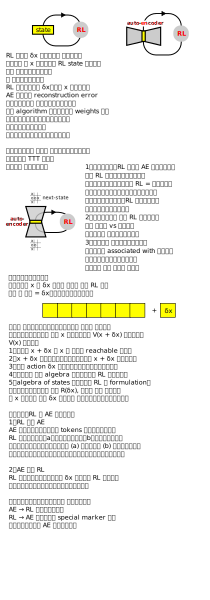
\includegraphics[scale=0.8]{RL-with-world-model.png}}}
\end{equation}
This is significant in physical environments, where physical actions are much more costly.  Ironically, most current AI training environments are already virtual, so this may not bring about large improvements.

\end{minipage}
\end{preview}

\begin{preview}
\begin{textblock*}{5cm}(2.1cm,2.3cm) % {block width} (coords) 
	{\color{red}{\large \textcircled{\small \themypage}}}
	\addtocounter{mypage}{1}
\end{textblock*}

\begin{minipage}{\textwidth}
	\setlength{\parskip}{0.4\baselineskip}

\section{Text world}

We want to find the ``path of least resistance'' to bootstrap an AGI.  Riding on the success of LLMs, we may want to train AGIs on a purely text-based environment.

An auto-encoder such as BERT would read a text and produce a latent representation (which could be in natural language, as NL is also a form of symbolic logic in a general sense).

The latent representation is the ``working memory'' of the intelligent system and its representation is more efficient for inferences than raw input.

The actor-critic of RL works in the latent representation (ie, a \textbf{model} of the world, taking virtual actions).  When a good virtual action is found, the algorithm would output an actual action.

\section{RL as ``thinking''}

Why take so much trouble to combine RL and LLM?  The benefit is that RL will find a way to optimize its internal ``thinking'' to achieve \textbf{logic coherence}.  This will cure the problem of LLM \textbf{hallucinations}.

This is feasible if we include ``thinking'' as ``\textbf{mental actions}'' in RL:
\begin{equation}
\vcenter{\hbox{\includegraphics[scale=0.8]{RL-outputs-thought-action.png}}}
\end{equation}

\end{minipage}
\end{preview}

\end{document}
